\section{Felhasználói követelmények}

A Sapi3D alkalmazás web alapú, ezért mindenki számára elérhető
a fő célja, hogy egy 3D modellként jelenítse meg a Sapientia EMTE Marosvásárhely-i karának a fő épületét, illetve ennek fontosabb helyeit, mint pl. tanszékek, titkárság stb. A rendszer fontosabb funkcionalitásait és az ezeket igénybe vevő szerepköröket a \ref{fig:UseCase} ábra szemlélteti.

Az elkészített alkalmazást bárki eltudja érni bárhonnan. Egyetlen feltételnek kell eleget tenni, amely az internet kapcsolat megvalósítása lenne. A rendszer megértésének érdekében tekintsük meg a \ref{fig:UseCase} ábrát amely bemutatja a rendszert, amit három különböző felhasználó vehet igénybe. A következő felhasználói szerepkörök vannak: VISITOR, USER és ADMIN. A három típusú felhasználó közül kettőnek van leheteősége bejelentkezésre (ADMIN, USER).

Az első szerepkör a VISITOR(látogató), amelynek lehetősége van megtekinteni az elkészített weboldalt, tudja használni a "vigyél el" opciót és nem utolsó sorban saját kezűleg is végig tud menni az egyetem 3D modelljén. Vannak olyen VISITOR-ok aki betudnak jelentkezni így átalakulnak USER-ré. A második szerepkör a USER, aki felelős az alkalmazás karbantartásáért is. A harmadik szerepkör az ADMIN. Az admin felhasználó akinek az egész rendszerben van a legnagyobb felelőssége. Ő felel azért, hogy mely visitorok kaphatnak engedélyt a bejelentkezéshez. Ez mellett az ő hatáskörébe tartozik, hogy ki lesz kitörölve a rendszerből. Mindezek mellet az admin joggal rendelkező felhasználó is felelős az alkalmazás karbantartásában. A karbantartás alatt kell érteni azt, hogy az oldalon megjelenő információk napra készek legyenek.
\begin{figure}[H]
	\centering
	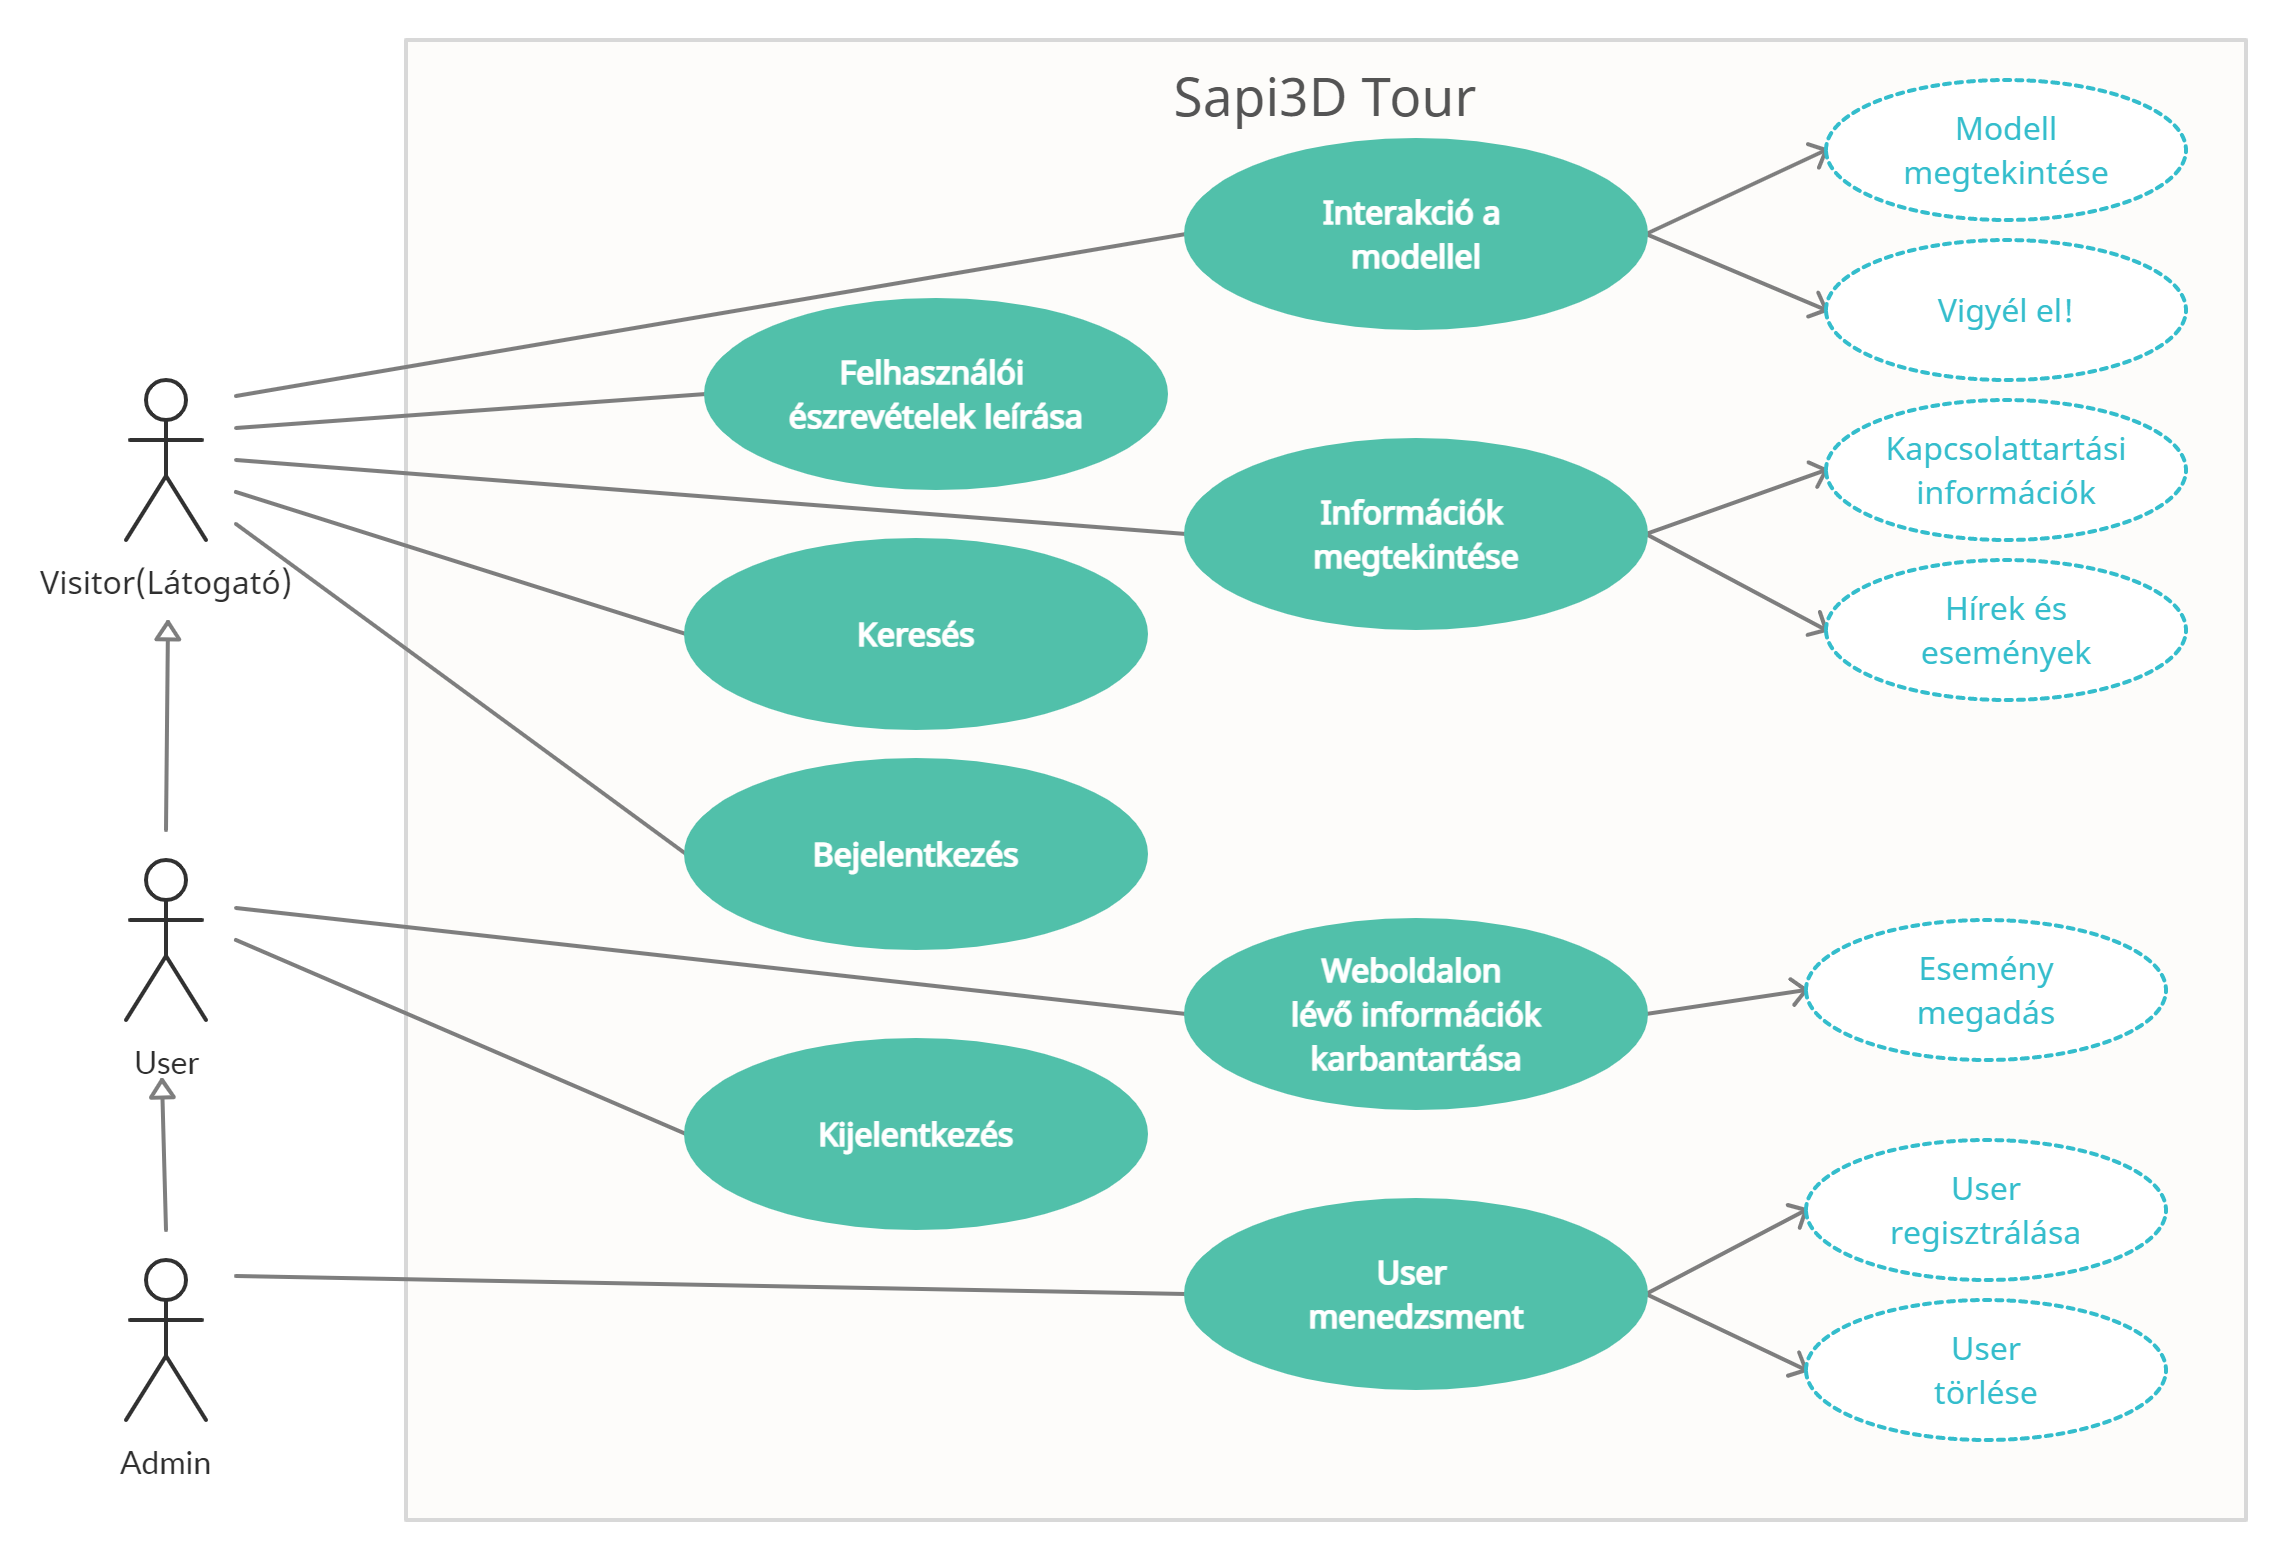
\includegraphics[width=1\linewidth]{figures/images/Sapi3dTourUseCase.png}
	\caption[A rendszer használati eset diagramja]{\textit{A rendszer használati eset diagramja}}
	\label{fig:UseCase}
\end{figure}

Bármely felhasználó, aki egy böngészőből megnyitja az oldalt, a VISITOR kategóriába kerül. Ez a fajta felhasználó megtekintheti a 3d modellt, körbe sétálhatja és el tud jutni pl.titkárságra. Amint megnyílt az oldal rögtön látható az egyetemről készített modell. Ezen a modellen tud nézelődni, esetleg körbe is tudja járni, vagy adott helységekre el is tud jutni(például: titkárság, adott tanszék). Ezen kívül lehetősége van információk, elérhetőségek, események részleteinek elolvasására is. Minden VISITOR ugyan akkor leírhatja saját véleményét, meglátásait az oldallal kapcsolatban is. A fent említett műveletek elvégzéséhez nem kell sem bejelentkezés, sem regisztráció.

Amennyiben a VISITOR bejelentkezik átkerül a USER kategóriába. A bejelentkezéshes szükséges megadni egy már regisztrált e-mail címet és egy már hitelesített jelszót is. A USER engedélyezése nem regszitráció alapján történik, hanem az admin joggal rendelkezők osztják ki, mivel a rendszer úgy van megtervezve, hogy nincs direkt regisztráció, hanem csak egy ADMIN tudja beregisztrálni az új USER-eket. Egy USER képes különböző műveletek elvégzésére, mint például: eseményeket megadni, az egyetemmel kapcsolatos információkat módosítani. Ezeken kívül mivel a VISITOR-ból lesz USER, így a USER-ből is tud lenni VISITOR a kijelentkezési opció esetén.

A regisztrációs feladatot egy admin jogosultsággal rendelkező felhasználó végezheti el. Nem csak a regisztrálás tartozik ehhez a feladatkörhöz, hanem a userek törlése is az ő feladata. Ezen plusz műveletek mellett szintén elvégezheti a USER és a VISITOR műveleteit is.